\documentclass{article}
\usepackage{../../fasy-hw}

\title{Computational Geometry, Homework \hwnum}
\collab{n/a}

%% Instructor: update these macros:
\renewcommand{\hwnum}{3}
\date{due: 9 March 2023}

%% Student: update this macro:
\author{\todo{Your Name Here}}

\begin{document}

\maketitle

This homework assignment should be
submitted as a single PDF file to D2L.

General homework expectations:
\begin{itemize}
    \item Homework should be typeset using LaTex.
    \item Answers should be in complete sentences and proofread so that they
        make sense without seeing the question.
    \item You will not plagiarize, nor will you share your written solutions
        with classmates. (But, discussing the questions is highly encouraged).
    \item List collaborators at the start of each question using the
        \texttt{collab} command.
    \item Put your answers where the \texttt{todo} command currently is (and
        remove the \texttt{todo} macro, but not the word \texttt{Answer}).
    \item If you are asked to come up with an algorithm, you are
        expected to give an efficient algorithm (brute-force solutions will not
        be accepted). With your algorithm, please provide the following:
        \begin{itemize}
            \item \emph{What}: A prose explanation of the problem and the algorithm,
                including a description of the input/output.  Be sure to state
                your GP assumptions.
            \item \emph{How}: Describe how the algorithm works clearly.
                Including pseudocode may helpful.
            \item \emph{How Fast}: Runtime, along with the derivation.  (Or, at
                the very least, a proof of termination using a decrementing
                function).  You only need to specify the space complexity if the
                problem asks for it.
           \item \emph{Why}: Brief justification of why the algorithm works.
               Often, this will include a statement of the loop invariant for each
               (outer-most) loop, or recursion invariant for each recursive function.
        \end{itemize}
\end{itemize}

{\bf David Mount's tips for writing up homework solutions}:
Remember that your description is intended to be read by a
human, not a compiler, so conciseness and clarity are preferred over technical
details.  Unless otherwise stated, you may use any results from class, or
results from any standard textbook on algorithms and data structures. Also, you
may use results from geometry that: (1) have been mentioned in class, (2) would
be known to someone who knows basic geometry or linear algebra, or (3) is
intuitively obvious. If you are unsure, please feel free to check with me.

Giving careful and rigorous proofs can be quite cumbersome in geometry, and so
you are encouraged to use intuition and give illustrations whenever appropriate.
Beware, however, that a poorly drawn figure can make certain erroneous
hypotheses appear to be ``obviously correct.''

Throughout the semester, unless otherwise stated, you may assume that input
objects are in general position. For example, you may assume that no two points
have the same x-coordinate, no three points are collinear, no four points are
co-circular. Also, unless otherwise stated, you may assume that any geometric
primitive involving a constant number of objects each of constant complexity can
be computed in $\Theta(1)$ time


{\bf Acknowledgement}: the homework problems were adapted from assignments of David
Millman, which, in turn, were adaptations of problems by David Mount and Carola
Wenk.

%%%%%%%%%%%%%%%%%%%%%%%%%%%%%%%%%%%%%%%%%%%%%%%%%%%%%%%%%%%%%%%%%%%%%%%%%%%%%%
\collab{\todo{}}
\nextprob{Dual Graph}

Let $P$ be a polygon in $\R^2$.  Suppose $P$ has $n$ vertices.
How many vertices, edges, and triangles does the dual graph of a frugal triangulation of $P$
have?  (Note: do not include a vertex for the outer face in the dual).  Be sure
to prove that your claim is correct.

\paragraph{Answer}

\todo{replace this TODO with your answer}
%%%%%%%%%%%%%%%%%%%%%%%%%%%%%%%%%%%%%%%%%%%%%%%%%%%%%%%%%%%%%%%%%%%%%%%%%%%%%%

%%%%%%%%%%%%%%%%%%%%%%%%%%%%%%%%%%%%%%%%%%%%%%%%%%%%%%%%%%%%%%%%%%%%%%%%%%%%%%
\collab{\todo{}}
\nextprob{Simple Polygonal Chain}

Given an polygonal chain $P$ of $n$ vertices, we define a vertex $v$ as a
\emph{local max} if $v$ all edges adjacent to $v$ are to the left of $v$.
Show that can determine if a polygonal chain with $k$ local maxes is simple in
$\Theta(n \log k)$ time.

\paragraph{Answer}

\todo{replace this TODO with your answer}
%%%%%%%%%%%%%%%%%%%%%%%%%%%%%%%%%%%%%%%%%%%%%%%%%%%%%%%%%%%%%%%%%%%%%%%%%%%%%%

%%%%%%%%%%%%%%%%%%%%%%%%%%%%%%%%%%%%%%%%%%%%%%%%%%%%%%%%%%%%%%%%%%%%%%%%%%%%%%
\collab{\todo{}}
\nextprob{River Flooding}

A friend of yours from the civil engineering department wants to analyze whether
a dangerous portion of a river will flood. He presents you with the following
(admittedly rather unrealistic) model of the river. The portion of the river of
interest is modeled as an $x$-monotone polygon $P$ that is bounded between two
vertical lines at $x = x^-$ and $x = x^+$ (see Figure). The river is bounded on
its left and right ends by two vertical line segments of lengths $w^-$ and
$w^+$, respectively. Inside the polygon are some number of disjoint x-monotone
polygons that represent islands in the river.  Let $n$ denote the total number
of vertices, including both the outer banks of the river and the islands.

\begin{figure}[h]
    \centering
    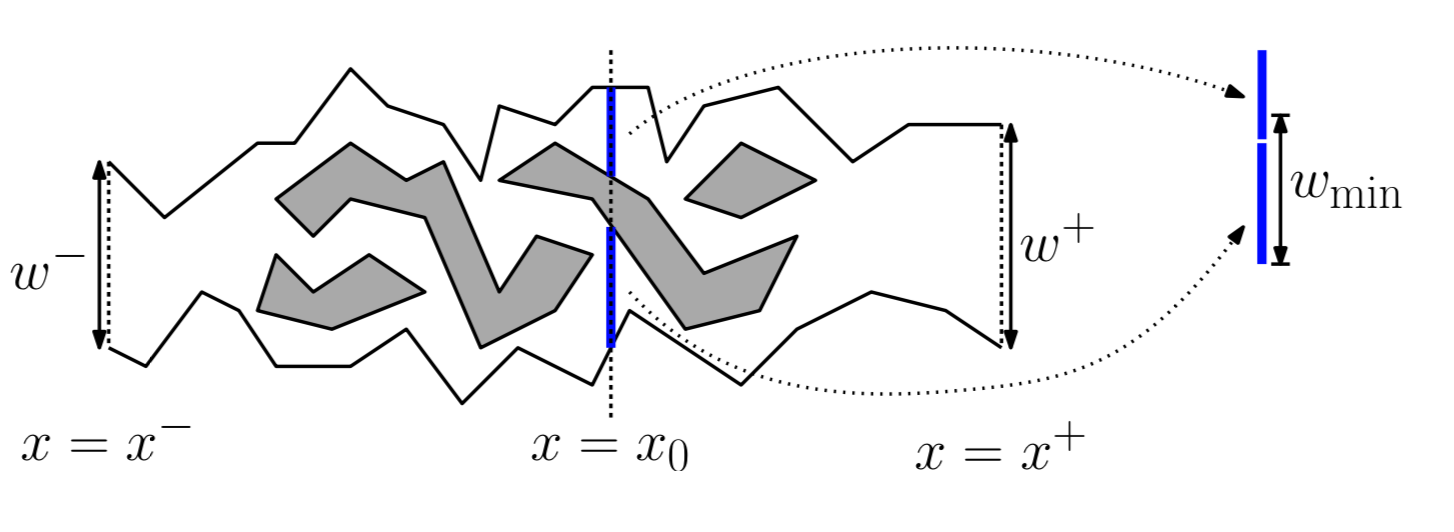
\includegraphics[width=0.75\textwidth]{river}
    \caption{River Flooding Problem}
\end{figure}

Your friend tells you that the in order to avoid a flood, the width of the river
(not counting islands) at every vertical cut must be at least some minimum value
$w_{min}$. For example, in the figure, the sum of the two blue vertical segments
at $x = x_0$ must be at least $w_{min}$ in order to avoid a flood.  Given the
polygon $P$ and the value $w_{min}$, present an $O(n \log n)$ time algorithm that
determines whether the river will flood, that is, whether there is a vertical
cut whose total width is smaller than $w_{min}$. If it will flood, your algorithm
should output the value $x_0$ of the bottleneck, that is, the location where the
sum of vertical lengths (excluding islands) is the smallest.

\begin{enumerate}
    \item Hint 1: There is an (uncountably) infinite number of possible vertical
        cuts to consider. Prove that it suffices to check the width at a
        at only a set of $\Theta(n)$ locations.

    \item Hint 2: There is a bit of a trick to updating the vertical widths
        (excluding the islands). For partial credit, explain how to do it under
        the assumption that the sweep line can only intersect a constant number
        of islands at any time. (For example, in the figure, the sweep line
        never hits more than two islands at a time.) For full credit, explain
        how to do it even if the number of islands hit by the sweep line at any
        time could be as high as $\Omega(n)$.
\end{enumerate}


\paragraph{Answer}

\todo{replace this TODO with your answer}
%%%%%%%%%%%%%%%%%%%%%%%%%%%%%%%%%%%%%%%%%%%%%%%%%%%%%%%%%%%%%%%%%%%%%%%%%%%%%%

%%%%%%%%%%%%%%%%%%%%%%%%%%%%%%%%%%%%%%%%%%%%%%%%%%%%%%%%%%%%%%%%%%%%%%%%%%%%%%
\collab{\todo{}}
\nextprob{Walk-Through}

Walk-through the algorithm for triangulating a polygon presented in DMLN L5 on
the following example.

\begin{figure}[h]
    \centering
    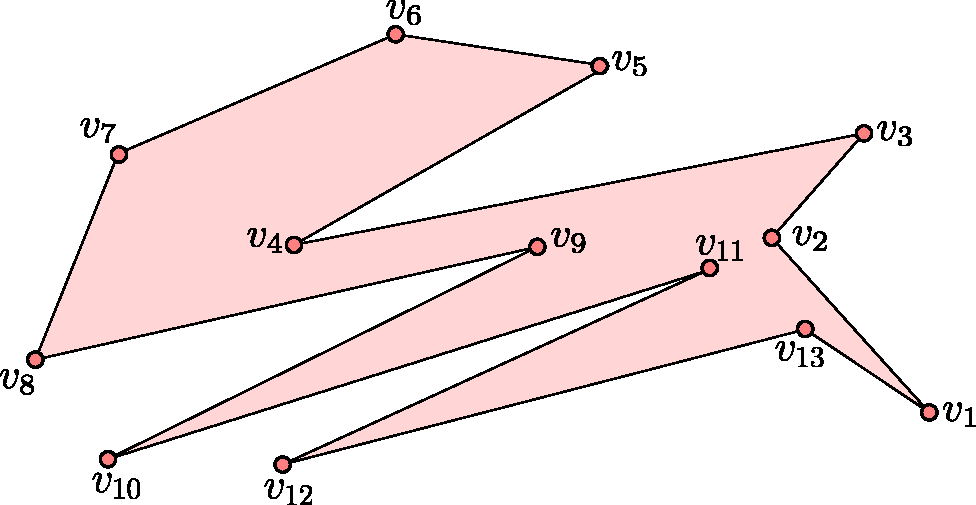
\includegraphics[width=0.75\textwidth]{polygon}
    \caption{Polygon}
\end{figure}

\paragraph{Answer}

\todo{replace this TODO with your answer}
%%%%%%%%%%%%%%%%%%%%%%%%%%%%%%%%%%%%%%%%%%%%%%%%%%%%%%%%%%%%%%%%%%%%%%%%%%%%%%

%%%%%%%%%%%%%%%%%%%%%%%%%%%%%%%%%%%%%%%%%%%%%%%%%%%%%%%%%%%%%%%%%%%%%%%%%%%%%%
\collab{\todo{}}
\nextprob{Reflection}

Explain to me anything that you tried differently on this homework, focused on
for improvement of technical writing, or what you would especially like feedback
on.  It can be something simple like ``Before this class, I was not very aware
of what tense I was writing in.  For this homework, I tried to focus on writing
in present tense.'' or something very focused, such as ``I really focused on
improving my End-condition proofs for loop invariants.''  If you tried something
and struggled, let me know. Since everyone needs to improve (including me),
there should be something that you can write about here.  You can base it on
feedback I gave you, feedback I gave the class, feedback you received from
someone else, an example of technical writing that you really liked, or anything
else that motivates you to improve.

\paragraph{Answer}

\todo{replace this TODO with your answer}
%%%%%%%%%%%%%%%%%%%%%%%%%%%%%%%%%%%%%%%%%%%%%%%%%%%%%%%%%%%%%%%%%%%%%%%%%%%%%%

\end{document}
